% !TeX spellcheck = en_GB
\ifcsname SlidesDistr\endcsname%
\documentclass[handout,aspectratio=169]{beamer}
\else%
\documentclass[aspectratio=169]{beamer}
\fi%
\input{../syde556_lecture_slides_preamble}


\usepackage{ragged2e}

\date{Nov 4, 2022}
\title{SYDE 556/750 \\ Simulating Neurobiological Systems \\ Lecture 9: Analysing Representations}

\begin{document}
	
	\begin{frame}{}
		\vspace{0.5cm}
		\begin{columns}[c]
			\column{0.6\textwidth}
			\MakeTitle
			\column{0.4\textwidth}
			\includegraphics[width=\textwidth]{media/maurice_denis_homage_to_cezanne_1900_small.jpg}
		\end{columns}
	\end{frame}

	\begin{frame}{Decoding Polynomials}
		\centering
		\includegraphics[width=\textwidth]{media/poly_decodings.pdf} 
	\end{frame}

  \begin{frame}{Projection of the Neuron Space to PCA}
    \centering
    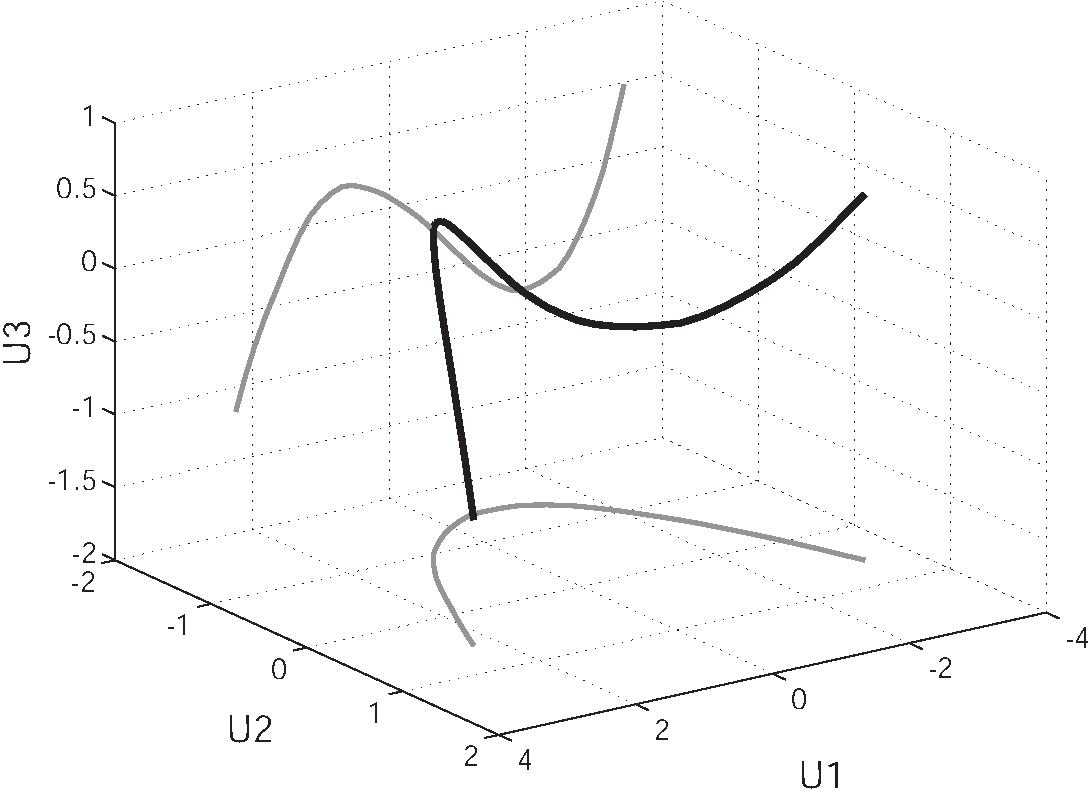
\includegraphics[scale=.4]{media/c5.chi.projections.pdf}
    
    A subspace of neuron activity being projected onto the first few principle component planes. Notice that the axis scales are different, capturing the size of the singular value.
  \end{frame}

	\begin{frame}{LIF Tuning Curve Principal Components}
		\centering
		\includegraphics[width=\textwidth]{media/tuning_curve_lif_pca.pdf}
		\begin{overlayarea}{\textwidth}{0.5cm}
			\centering
		\end{overlayarea}
	\end{frame}

	\begin{frame}{ReLU Tuning Curve Principal Components}
		\centering
		\includegraphics[width=\textwidth]{media/tuning_curve_relu_pca.pdf}
		\begin{overlayarea}{\textwidth}{0.5cm}
			\centering
			\only<2->{\hl{$\approx$ Legendre Basis}}
		\end{overlayarea}
	\end{frame}

	\begin{frame}{Reminder: Legendre Polynomials}
		\centering
		\includegraphics{media/legendre.pdf}
		\begin{align*}
			\phi_i(x)&= \frac{1}{2^i} \sum_{k=0}^n \binom{i}{k}^2 (x-1)^{i-k}(x+1)^k
		\end{align*}
		\begin{overlayarea}{\textwidth}{0.5cm}
			\centering
		\end{overlayarea}
	\end{frame}

	\begin{frame}{Modifying the Basis -- Same Maximum Rate (I)}
		\centering%
		\includegraphics<1>[width=\textwidth]{media/tuning_curve_relu_pca.pdf}%
		\includegraphics<2->[width=\textwidth]{media/tuning_curve_relu_pca_fix_max_rate.pdf}
		\begin{overlayarea}{\textwidth}{0.5cm}
			\centering
		\end{overlayarea}
	\end{frame}


	\begin{frame}{Modifying the Basis -- Equidistant $x$-Intercepts (II)}
		\centering%
		\includegraphics[width=\textwidth]{media/tuning_curve_relu_pca_fix_max_rate_intercepts_i.pdf}
		\begin{overlayarea}{\textwidth}{0.5cm}
			\centering
		\end{overlayarea}
	\end{frame}

	\begin{frame}{Modifying the Basis -- Limited $x$-Intercepts (III)}
		\centering%
		\includegraphics[width=\textwidth]{media/tuning_curve_relu_pca_fix_max_rate_intercepts_ii.pdf}
		\begin{overlayarea}{\textwidth}{0.5cm}
			\centering
		\end{overlayarea}
	\end{frame}

	\begin{frame}{Modifying the Basis -- Symmetric Tuning Curves (IV)}
		\centering%
		\includegraphics[width=\textwidth]{media/tuning_curve_relu_pca_symmetric.pdf}
		\begin{overlayarea}{\textwidth}{0.5cm}
			\centering
		\end{overlayarea}
	\end{frame}

	\begin{frame}{Gaussian Tuning Curve Principal Components}
		\centering
		\includegraphics[width=\textwidth]{media/tuning_curve_gaussian_pca.pdf}
		\begin{overlayarea}{\textwidth}{0.5cm}
			\centering
			\only<2->{\hl{$\approx$ Fourier Basis}}
		\end{overlayarea}
	\end{frame}

  \begin{frame}{Gaussian vs LIF Singular Values}
		\centering
		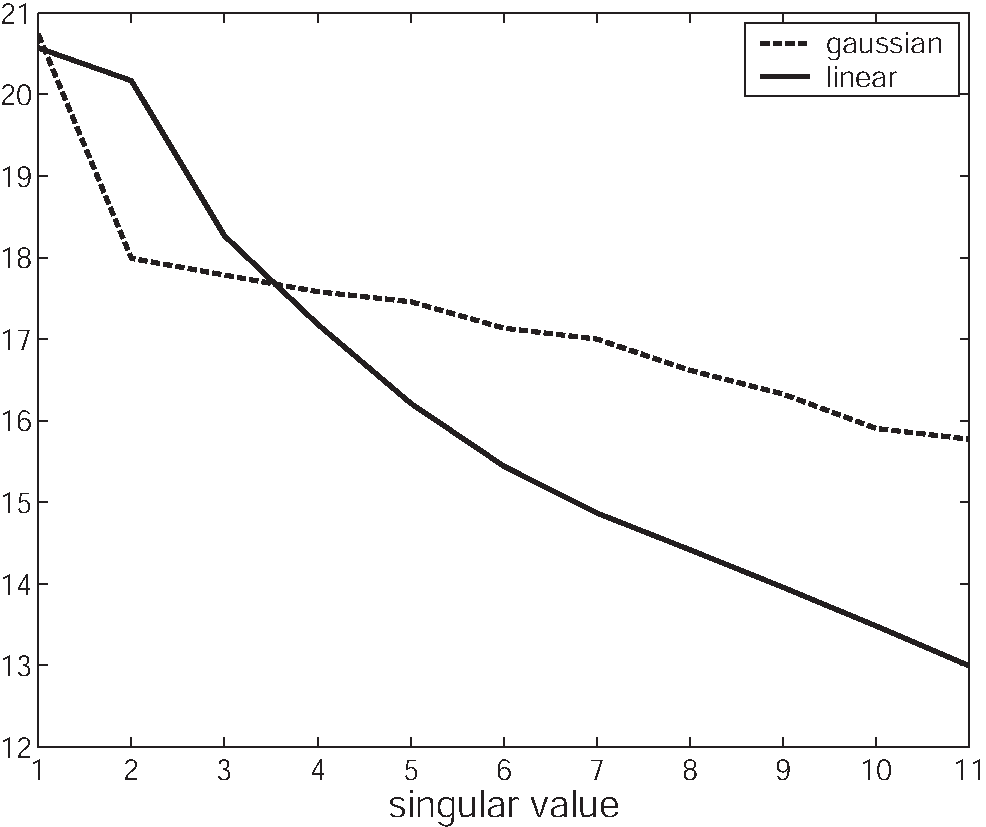
\includegraphics[scale=.5]{media/c5.line.gauss.sing.vals.pdf}
	\end{frame}

	\begin{frame}{PCA of 2D Tuning Curves}
		\centering
		\includegraphics[width=\textwidth]{media/2d_tuning_curves.pdf}
		\begin{overlayarea}{\textwidth}{0.5cm}
			\centering
			\only<2->{\vspace*{-0.5cm}\hl{Combination of 2D Polynomials}}
		\end{overlayarea}
	\end{frame}

  \begin{frame}{2D Singular Values}
		\centering
		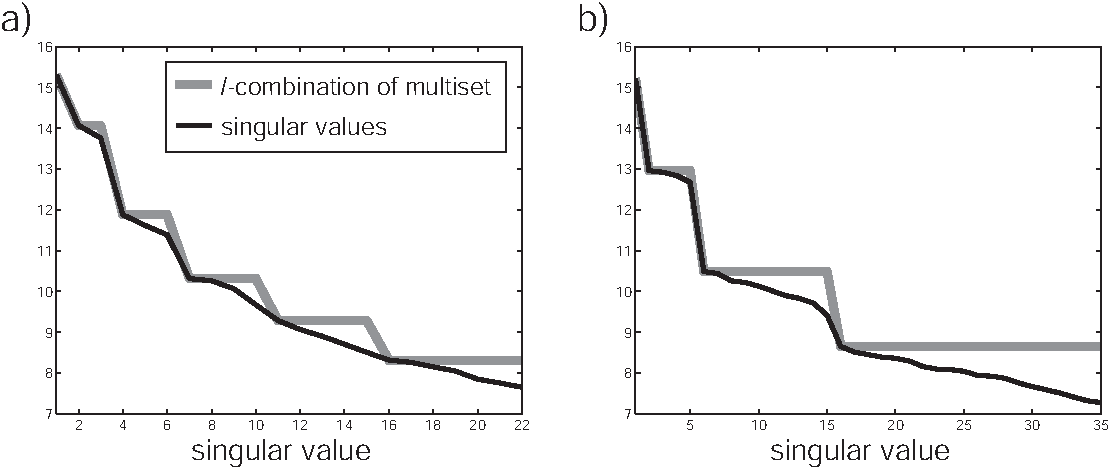
\includegraphics[scale=.5]{media/c5.multiset.2D.pdf}

    2D and 4D singular values compared to the prediction of the multiset (i.e., number of cross terms).
	\end{frame}

	\begin{frame}{Conclusions}
		\begin{itemize}
			\setlength{\itemsep}{0.5cm}
			\item Can use \hl{PCA} to find the basis functions underlying neural representations
			\item \hl{Singular values} inversely proportional to noise
			\item \hl{Basis function shape} depends on\\[0.25cm]
			\begin{itemize}
				\setlength{\itemsep}{0.25cm}
				\item $x$-intercept distributions
				\item Neuron response curve $G[J]$
			\end{itemize}
			\item Finding optimal tuning curves for computing particular functions\\
			$\Rightarrow$ Full network optimization (must use gradient descent)
		\end{itemize}
	\end{frame}

	\backupbegin

	\begin{frame}[noframenumbering]{Image sources}
		\small
		\textbf{Title slide}\\Maurice Denis: Homage to Cézanne, 1900\\From \href{https://commons.wikimedia.org/wiki/File:Maurice_Denis_Homage_to_Cezanne_1900.jpg}{Wikimedia}.
	\end{frame}

	\backupend
	
\end{document}
